% 1000 words
\section*{}
To recapitulate our findings thus far: First, we have established that provided with open data on population, amenity points-of-interest density and diversity, and public transportation accessibility indices, we can predict the total number of arrivals by public transport to a high degree of accuracy using an XGBoost model that is fine-tuned to overcome overfitting. Secondly, using SHAP for machine learning model explanation, we managed to extract more sophisticated feature importance indications than originally available with XGBoost. Furthermore, by examining local SHAP explanations, we can identify hotspots for different POI features overall and across different time bands, together with its shortcomings. 

One of the benefits of using SHAP values as imperfect approximants to coefficients in a statistical model is their additive nature. This means that we can decompose the model's predictions into the sum of the SHAP values, with which we can control for unwanted effects. For example, without an explicit origin-destination matrix and dwell time data and using only station exits and bus alighting data, it is not immediately possible to say whether a person is exiting at a destination to attend an activity or to interchange to another mode of transport. Using SHAP to extract local importance with its additive property can help consider the impact of the amenity profile of the destination area on the trip attractiveness of the area while controlling for the connectivity profile of the area. 

\begin{figure}[!ht]
    \centering
    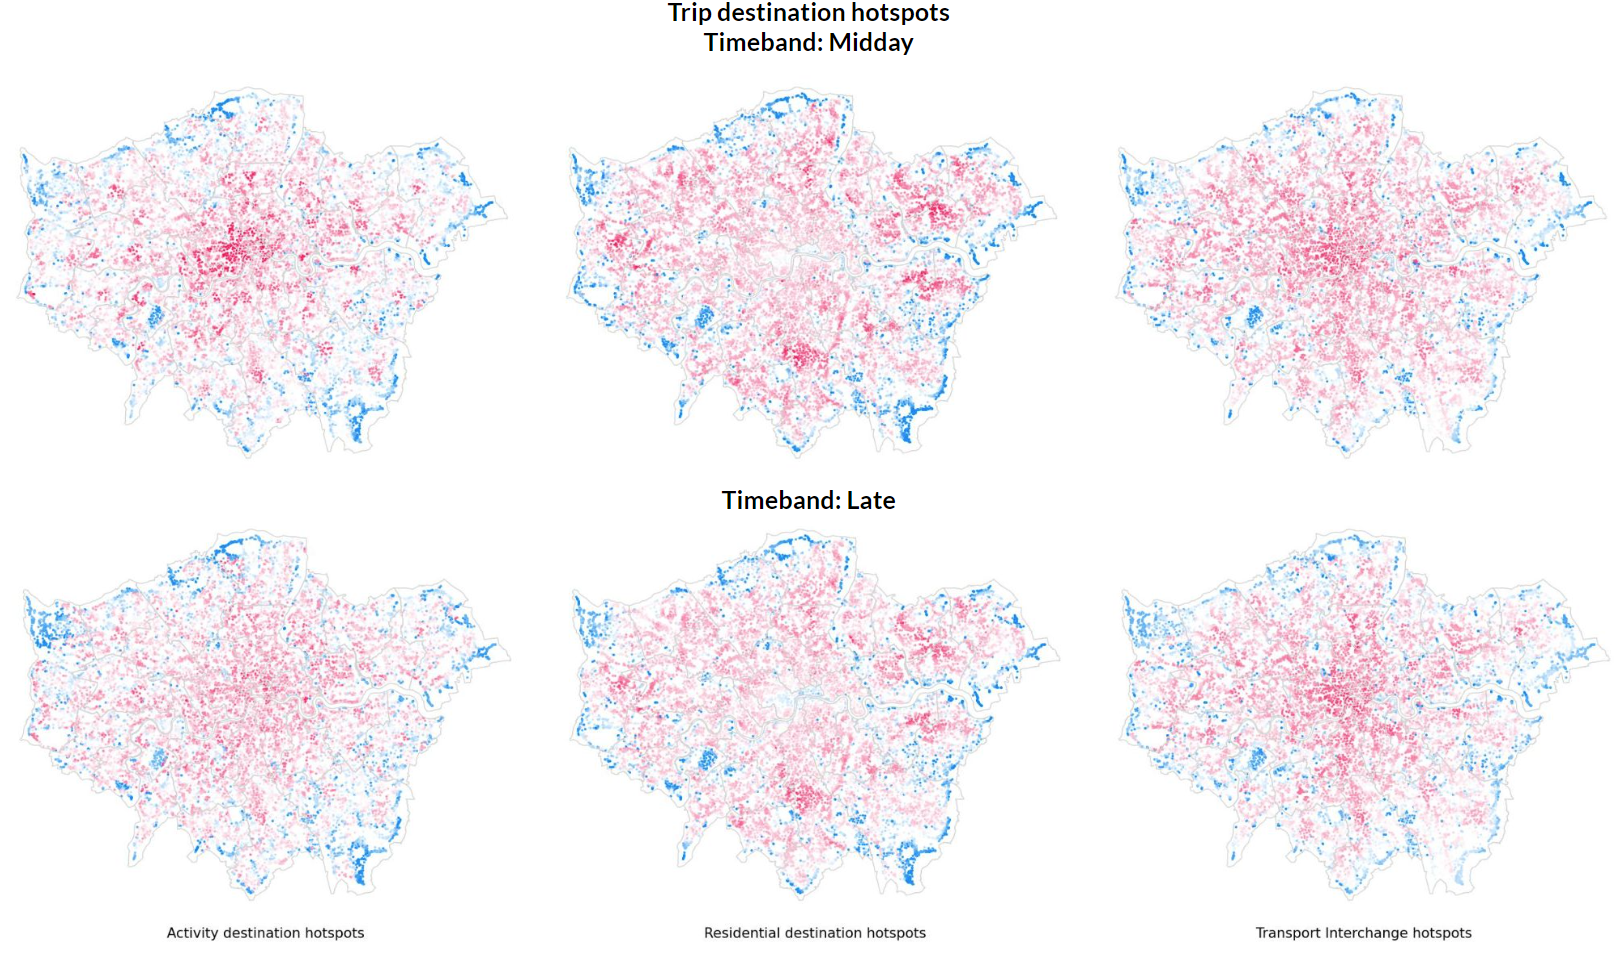
\includegraphics[width=0.75\textwidth]{destinationhotspot.png}
    \captionsetup{justification=centering}
    \caption{Hot spots for destination groups: Amenity vs. Residential vs. Transport\\ Midday vs Late}
    \label{fig:destinationhotspot}
\end{figure}

One way to visualise it is by grouping local SHAP values by feature groups and visualising their spatial distribution. This can be seen in Figure \ref{fig:destinationhotspot} with features grouped into (1) amenity-related, (2) population, and (3) connectivity-related features. When comparing Midday and Late time bands, representing the peak and lowest volumes respectively, we can see that the trip attractiveness of areas because of their connectivity profile is unchanged, whereas the trip attractiveness of areas because of their amenity profile is significantly more pronounced in the Midday time band, despite the fact that connectivity-related features have high global importance. With the hypothesis that the only difference between these two time bands are the trip attraction generated by amenities as destination, this suggests that when grouped in this manner, the model as the whole seems to be able to isolate whether an area is attractive because of their amenities or their connectivity in the network. 

This is useful for instances where we want to qualify certain popular areas as destination hotspots based on the availability of amenities alone while disregarding their connectivity-based attractors. Applying spatial clustering such as HDBSCAN of spatial units based on their amenity-related compound SHAP values can effectively surface activity hotspots in a given area in Greater London. Figure \ref{fig:woodgreen} demonstrates the activity hotspot in Wood Green with the highest mean amenity-related compound SHAP values, made up of 5 constituent spatial units (isochrones). This can be useful for local urban planners to identify destination areas that are popular for non-commute activities, such as parks, shopping, dining, or entertainment.

\begin{figure}[!ht]
    \centering
    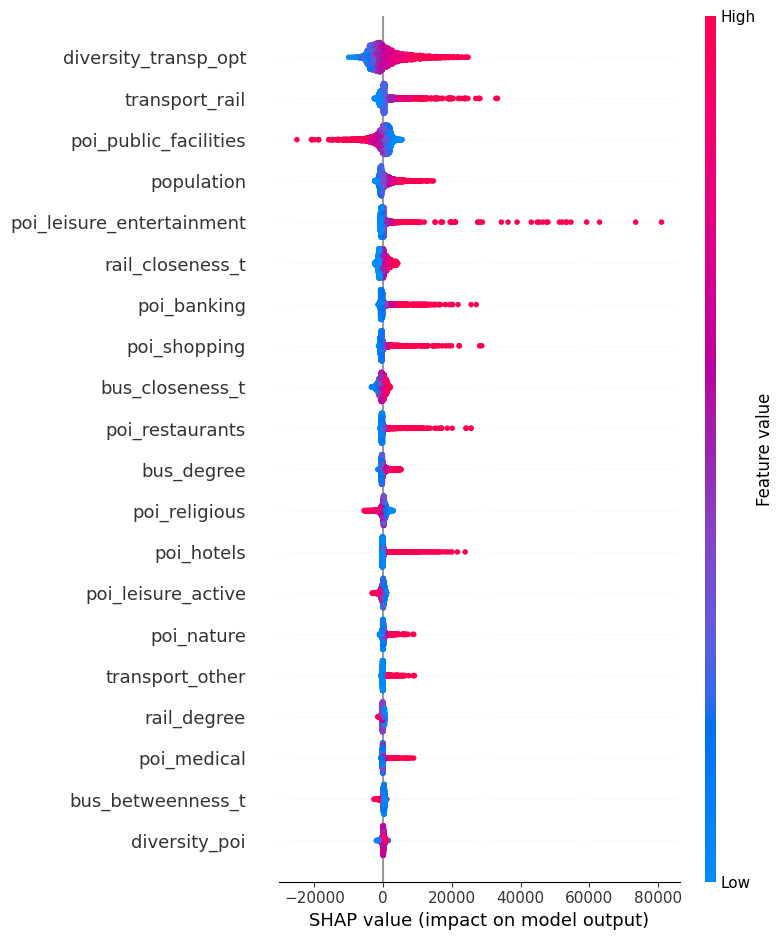
\includegraphics[width=0.8\textwidth]{output.png}
    \captionsetup{justification=centering}
    \caption{Identifying high activity areas in Wood Green}
    \label{fig:woodgreen}
\end{figure}

Finally, it is worth acknowledging the methodology's limitations, which affect its generalisability and applicability in certain cases.

\begin{itemize}
    \setlength\itemsep{0em}
    \item \textit{Core assumptions on target variable selection}: In order to approximate non-commute trip attractiveness, we opted for data on a Saturday as a typical weekend day to remove the effect of employment centres from the analysis as much as possible. However, this does not account for travel demand from those who work on weekends. 
    \item \textit{Missing features}: The analysis of outliers suggests that there are other factors that may be influencing the number of arrivals in an area that are not accounted for in the model. These could include socioeconomic factors, car ownership, or other urban morphological features that affect people's usage of public transport.
    \item \textit{Generalisability}: The high feature importance of the spatial lag features across the board means that the model may not be able to accurately predict a new observation in isolation from its neighbours, nor can it be readily generalisable to other cities. Nevertheless, the model can be used to predict the trip attractiveness of a given area in Greater London as the city changes, giving transport planners a useful tool. For example, when a neighbourhood is undergoing redevelopment, we can predict the potential inflow of public transport trips based on the planned addition of amenities or transport facilities.
    \item \textit{Causality}: However, the lack of consideration for causality means that we cannot infer that the presence of a certain amenity of a certain density will cause more arrivals to a certain area. Rather, we can only make predictions of potential trips attracted based on the presence of certain amenities.
    \item \textit{POI classification}: The classification of amenity and transport POIs in this analysis adheres to Geofabrik's out-of-the-box OSM data classification. Future work could attempt to reclassify these POIs in a deliberate manner to capture the association between certain trip purposes of interest and the types of amenities that fulfil them as destinations.
\end{itemize}

Last but not least, the scope of the dissertation is limited to public transport trips and does not account for other types of mobility, such as cycling, walking, or driving, which may be more prevalent on weekends, which would provide a more comprehensive understanding of the non-commute trip attractiveness of an area regardless of mode of transport, and during time bands when public transport is less accessible such as late nights. Future work could incorporate mode-agnostic mobility data together with trip purpose inferences into a modified version of this methodology to provide a more comprehensive understanding of what draws people to a certain area in Greater London. Special care should be taken to ensure that the chosen features reflect the trip purposes and the transport modes of interest.